\documentclass[10pt,journal]{IEEEtran}

\usepackage{amsmath,amssymb}
\usepackage{graphicx}
\usepackage{booktabs}
\usepackage{array}
\usepackage[hidelinks]{hyperref}
\usepackage{microtype}
\usepackage{newunicodechar}

\graphicspath{{figures/}{../figures/}}

% --- Unicode mappings so this compiles under pdflatex (arXiv default) ---
\newunicodechar{—}{---}
\newunicodechar{–}{--}
\newunicodechar{−}{\ensuremath{-}}
\newunicodechar{→}{\ensuremath{\rightarrow}}
\newunicodechar{Δ}{\ensuremath{\Delta}}
\newunicodechar{±}{\ensuremath{\pm}}
\newunicodechar{×}{\ensuremath{\times}}
\newunicodechar{…}{\ldots}
\newunicodechar{∈}{\ensuremath{\in}}
\newunicodechar{≤}{\ensuremath{\leq}}
\newunicodechar{≥}{\ensuremath{\geq}}
\newunicodechar{≈}{\ensuremath{\approx}}
\newunicodechar{≫}{\ensuremath{\gg}}
\newunicodechar{·}{\textperiodcentered}
\newunicodechar{μ}{\ensuremath{\mu}}
\newunicodechar{✓}{\checkmark}
\newunicodechar{✗}{\ensuremath{\times}}

\begin{document}

\title{Fast and Faithful? Distilling an 8B Reasoning Teacher into a Sub-1B On-Device Student for Structured News Enrichment}

\author{Vinay~Kumar~Chaganti% <-this % stops a space
\thanks{The author is an independent researcher (e-mail: cvk.atreya@gmail.com).}%
\thanks{Evaluation-harness code, figure-generation scripts, and portions of the manuscript were produced with AI-agent assistance; see the Acknowledgment.}}

\markboth{Preprint, July 2026}{Chaganti: Distilling an 8B Reasoning Teacher into a Sub-1B On-Device Student}

\maketitle

\begin{abstract}
What does knowledge distillation actually buy a production pipeline, measured per sub-task, against the cheaper levers a practitioner would try first? This is quantified on a real, shipped deployment: an RSS reader that enriches each article with one structured JSON object---a free-text summary, five categorical labels, and open-set topics---at the output quality of an 8B reasoning teacher (\texttt{deepseek-r1:8b}) but without its {\raise.17ex\hbox{$\scriptstyle\sim$}}39 s/article latency. A 600M student (Qwen3-0.6B) is fine-tuned on the teacher's outputs (QLoRA, three seeds) and scored per sub-task against two non-distillation controls---few-shot prompting and constrained JSON decoding---and a managed-platform distillation pipeline, by a blinded, reference-free, two-judge panel grading against the full article. The answer is per-field. Speed is a property of size, not distillation: every 0.6B arm runs at {\raise.17ex\hbox{$\scriptstyle\sim$}}0.8 s/article. Summary quality is where distillation earns its keep: the tuned student closes {\raise.17ex\hbox{$\scriptstyle\sim$}}59\% of the base-to-teacher gap and significantly beats both controls (+15.5 points over constrained decoding, +5.9 over few-shot). Classification splits field by field: the apparent urgency win over the teacher is mostly majority-class alignment, tone belongs to prompting, and the macro ties few-shot. Faithfulness shows a small deficit against the untuned base whose magnitude sits within the instrument's measured noise; what is robust is its concentration in short-source articles, where the student fabricates. A managed-platform pipeline ties the do-it-yourself recipe on summary quality with an inverted profile---the best small-model classifier, the worst thin-source faithfulness---so the two recipes transfer different capabilities. The deliverable is a per-field engine assignment: the smallest routed subset that pays, with a latency-priced teacher fallback for faithfulness-critical thin sources.
\end{abstract}

\begin{IEEEkeywords}
Edge inference, knowledge distillation, large language models, LLM-as-a-judge evaluation, model compression, small language models, structured output generation, text summarization.
\end{IEEEkeywords}

\section{Introduction}\label{sec:intro}
\IEEEPARstart{T}{his} study began as a quantification problem: before adopting distillation across a family of production tasks, one wants a defensible measurement of what it actually buys, per sub-task, against the cheaper levers a practitioner would try first. The task pattern under study---one prompt, one schema-bound JSON object per item, repeated over thousands of items---recurs across production pipelines (ticket triage, log classification, document intake, catalog extraction), so the lessons are expected to outlive the first application.

That first application is real and shipped: a local-first RSS reader\footnote{The deployment is a personal RSS reader; the product itself is incidental to this study and is named only for reproducibility of the corpus. The paper's claims concern the distillation and evaluation method, not the application.} that enriches every incoming article with a structured JSON object: a short analytical summary, five closed-vocabulary content-analysis labels---\emph{sentiment}, \emph{urgency}, \emph{frame}, \emph{tone}, \emph{depth}---and open-set topic tags (full vocabularies in Section~\ref{sec:task}). Generating that with the \texttt{deepseek-r1:8b} teacher produced acceptable output, but at {\raise.17ex\hbox{$\scriptstyle\sim$}}39 s/article; enriching a 500-article backlog was a 5.4-hour job on a consumer laptop (Fig.~\ref{fig:efficiency}, left). The engineering goal was to keep that output quality while making the batch fast enough to run locally as a routine, unattended job.

Running the study fully locally was itself a measurement decision, not only a deployment constraint. Free-tier hosted APIs proved too unreliable for controlled quantification---rate limits and dropped completions later constrained even the judge panel (Section~\ref{sec:judges})---whereas local models hold still: fixed weights, temperature 0, no quotas, unlimited reruns. Everything needed to re-measure is therefore local and free.

Two levers were available, and it is worth being precise about which does what, because the two are easily conflated. \emph{Model size buys speed}: a 0.6B model runs {\raise.17ex\hbox{$\scriptstyle\sim$}}40$\times$ faster than the 8B teacher regardless of how it was trained; this lever is free and was never in question. \emph{Distillation buys quality at that size}: it is the only lever that can make a 0.6B model produce output resembling the teacher's, and it is the lever under test. So the real question is not ``is the small model faster'' (trivially yes) nor ``was distillation worth it'' (worth it \emph{for what?}), but: how much of an 8B teacher's output quality can a 600M student recover through distillation, on each part of a structured task, and does it preserve the properties (faithfulness above all) that a reader-facing product cannot compromise?

A credible answer needs more than the obvious first cut---a single same-family judge, a handful of test items, a 0--5 rubric that saturates near the ceiling, and one training run. This study answers the question with a design built to resist each of those failure modes: 93 held-out test articles; eight arms including two non-distillation controls and a managed-platform distillation pipeline; a decomposition into three sub-tasks with different success criteria; a multi-family judge panel validated by a negative control; three training seeds; and paired-bootstrap significance tests. The summary rubric was fixed after a pilot and before any scored run, so it could not be tuned to the result.

The contributions are: (1) a fully local, reference-free, human-free evaluation harness for structured-output distillation, reproducible offline from a cached judge log; (2) gap-closure-to-teacher as a reporting scale matched to the engineering goal, which naturally exposes overshoot and regression; (3) a per-sub-task decomposition separating summarization, classification, and topic tagging, which reveals effects any aggregate score hides; (4) two non-distillation controls so distillation is credited only for what neither cheaper lever provides; and (5) a per-field engine assignment for on-device enrichment plus an explicit map of the build decisions the exercise required.

This paper does \emph{not} claim that the teacher's reasoning nature was necessary; it uses no human gold labels; it uses a two-judge panel, so exact magnitudes are not judge-invariant; and its classification ``accuracy'' is measured against a judge-panel consensus, not ground truth (Section~\ref{sec:limits}).

\section{Related Work}\label{sec:related}
\emph{Knowledge distillation.} Training a small student to imitate a larger teacher dates to Hinton \emph{et al.} \cite{hinton2015}, with sequence-level distillation for generation introduced by Kim and Rush \cite{kimrush2016}. The modern LLM variant---a large model generates outputs on which a smaller model is supervised-fine-tuned---is what surveys term black-box or sequence-level distillation \cite{xusurvey2024, zhu2023}. The pipeline here is a textbook instance; what distinguishes this study is not the method but the measurement: most distillation work reports a single aggregate quality delta, whereas this study decomposes by sub-task and controls for cheaper alternatives.

\emph{Rationale over labels.} A parallel line supervises the student on the teacher's reasoning, not just its answers. Distilling step-by-step \cite{hsieh2023} shows rationale supervision is more data-efficient than label-only; symbolic chain-of-thought distillation \cite{li2023} shows sub-1.3B students can absorb chain-of-thought. This study deliberately trains on the teacher's final outputs only (thinking disabled): these tasks are non-reasoning and it is the deployment-realistic recipe; whether trace supervision would help is left as future work.

\emph{Reasoning-teacher distillation.} DeepSeek-R1 \cite{deepseek2025} showed that distilling a strong reasoning model into smaller dense models transfers reasoning ability, triggering a wave of replication studies \cite{zhang2025}. That literature is almost entirely about math, code, and reasoning benchmarks at the 1.5B--32B scale. NaturalThoughts \cite{li2025} frames the answer-only versus trace distillation axis directly and studies equal-size non-reasoning students. The present setting sits in the gap that leaves: a reasoning teacher distilled into a sub-1B student for non-reasoning production tasks, where the recipe's value is contested rather than assumed.

\emph{Reasoning can hurt.} The assumption that a reasoning teacher helps is not safe for simple tasks. OptimalThinkingBench \cite{aggarwal2025} documents that thinking models distilled into non-thinking students can degrade on straightforward queries---``overthinking'' transfers through distillation. The faithfulness regression reported here (Section~\ref{sec:faithful}) is an independent data point in this direction.

\emph{Small models and their limits.} Qwen3 \cite{yang2025} is itself a strong-to-weak distillation product, and Qwen3-0.6B is at the low edge where chain-of-thought distillation is known to become unreliable. Speculative distillation \cite{xuspec2024} covers 0.5B-class students on summarization, but via on-policy methods and without the per-field, controlled decomposition used here.

\emph{Judging and faithfulness evaluation.} Scalar LLM judging \cite{liu2023, ye2023} is known to suffer positional, verbosity, and style biases and to saturate near the ceiling. The field's response is decomposition: checklist-based judging \cite{lee2024} and open-rubric judges \cite{kim2024}. For faithfulness, atomic-fact methods \cite{min2023, ru2024} and efficient local entailment checkers \cite{tang2024} replace $n$-gram overlap, and reference-free hallucination detection \cite{manakul2023} avoids gold references. The harness here adopts the checklist-decomposition and reference-free-validation lessons from this line while staying fully local and human-free.

\emph{What is being distilled.} \texttt{deepseek-r1:8b} is DeepSeek-R1-Distill-Llama-8B, itself a distilled dense model derived from the 671B R1 \cite{deepseek2025}, and Qwen3-0.6B is itself a distillation product. The pipeline is therefore third-order distillation, which caps the achievable ceiling (Section~\ref{sec:limits}).

\section{The Structured Enrichment Task}\label{sec:task}
The reader enriches every incoming article with one JSON object carrying seven fields: a free-text summary, five categorical labels, and an open-set topic list. These surface directly in the user interface as a content-analysis panel (Fig.~\ref{fig:panel}). A representative teacher output pairs a three-to-four-sentence summary with the label fields, e.g., \emph{sentiment}=positive, \emph{urgency}=developing, \emph{frame}=analytical, \emph{tone}=analytical, \emph{depth}=standard, and \emph{topics}=\{AI~Safety, Responsible~AI\}.

\begin{figure}[t]\centering

\includegraphics[width=\columnwidth]{fig1_panel.png}
\caption{The enrichment as the reader sees it. The five categorical fields and the topic tags render as badges in a content-analysis panel; the free-text summary is shown separately. A hallucinated summary misleads the reader, whereas a mislabelled badge is glanceable and cheap---the asymmetry that motivates the per-field engine assignment.}
\label{fig:panel}
\end{figure}

The categorical fields draw from small closed vocabularies observed in the teacher's own labels: \emph{sentiment} $\in$ \{positive, neutral, negative\}; \emph{urgency} $\in$ \{breaking, developing, evergreen\}; \emph{frame} $\in$ \{analytical, conflict, human\_interest, economic\}; \emph{tone} $\in$ \{analytical, optimistic, opinion, alarming\}; \emph{depth} $\in$ \{brief, standard, deep\_dive\}. Several vocabularies are imbalanced (e.g., \emph{depth}: 56\% standard, 26\% brief, 2\% deep\_dive), which matters directly for interpreting per-field accuracy and is made concrete with a majority-class baseline in Section~\ref{sec:classification}.

This single output is really three machine-learning problems with different success criteria (Table~\ref{tab:subtasks}), and scoring them together hides what distillation moved. The asymmetry in failure cost is why the study's conclusion is a per-field engine assignment (Section~\ref{sec:assignment}) rather than a single verdict: the quality bar a field must clear depends on what a wrong value costs.

\begin{table}[t]
\centering
\caption{The Enrichment Output Is Three Sub-Tasks With Different Failure Costs}
\label{tab:subtasks}
\small
\begin{tabular}{@{}p{1.7cm}p{1.9cm}p{3.2cm}@{}}
\toprule
Sub-task & Type & Failure cost in the product \\
\midrule
Summarization (\texttt{summary}) & free-text generation & high --- a hallucinated summary misleads \\
Classification (5 labels) & closed-set labels & low --- a mislabeled badge is cheap \\
Topic tagging (\texttt{topics}) & open-set multi-label & low --- affects filtering, not comprehension \\
\bottomrule
\end{tabular}
\end{table}

\section{Experimental Setup}\label{sec:setup}
\begin{figure*}[t]\centering
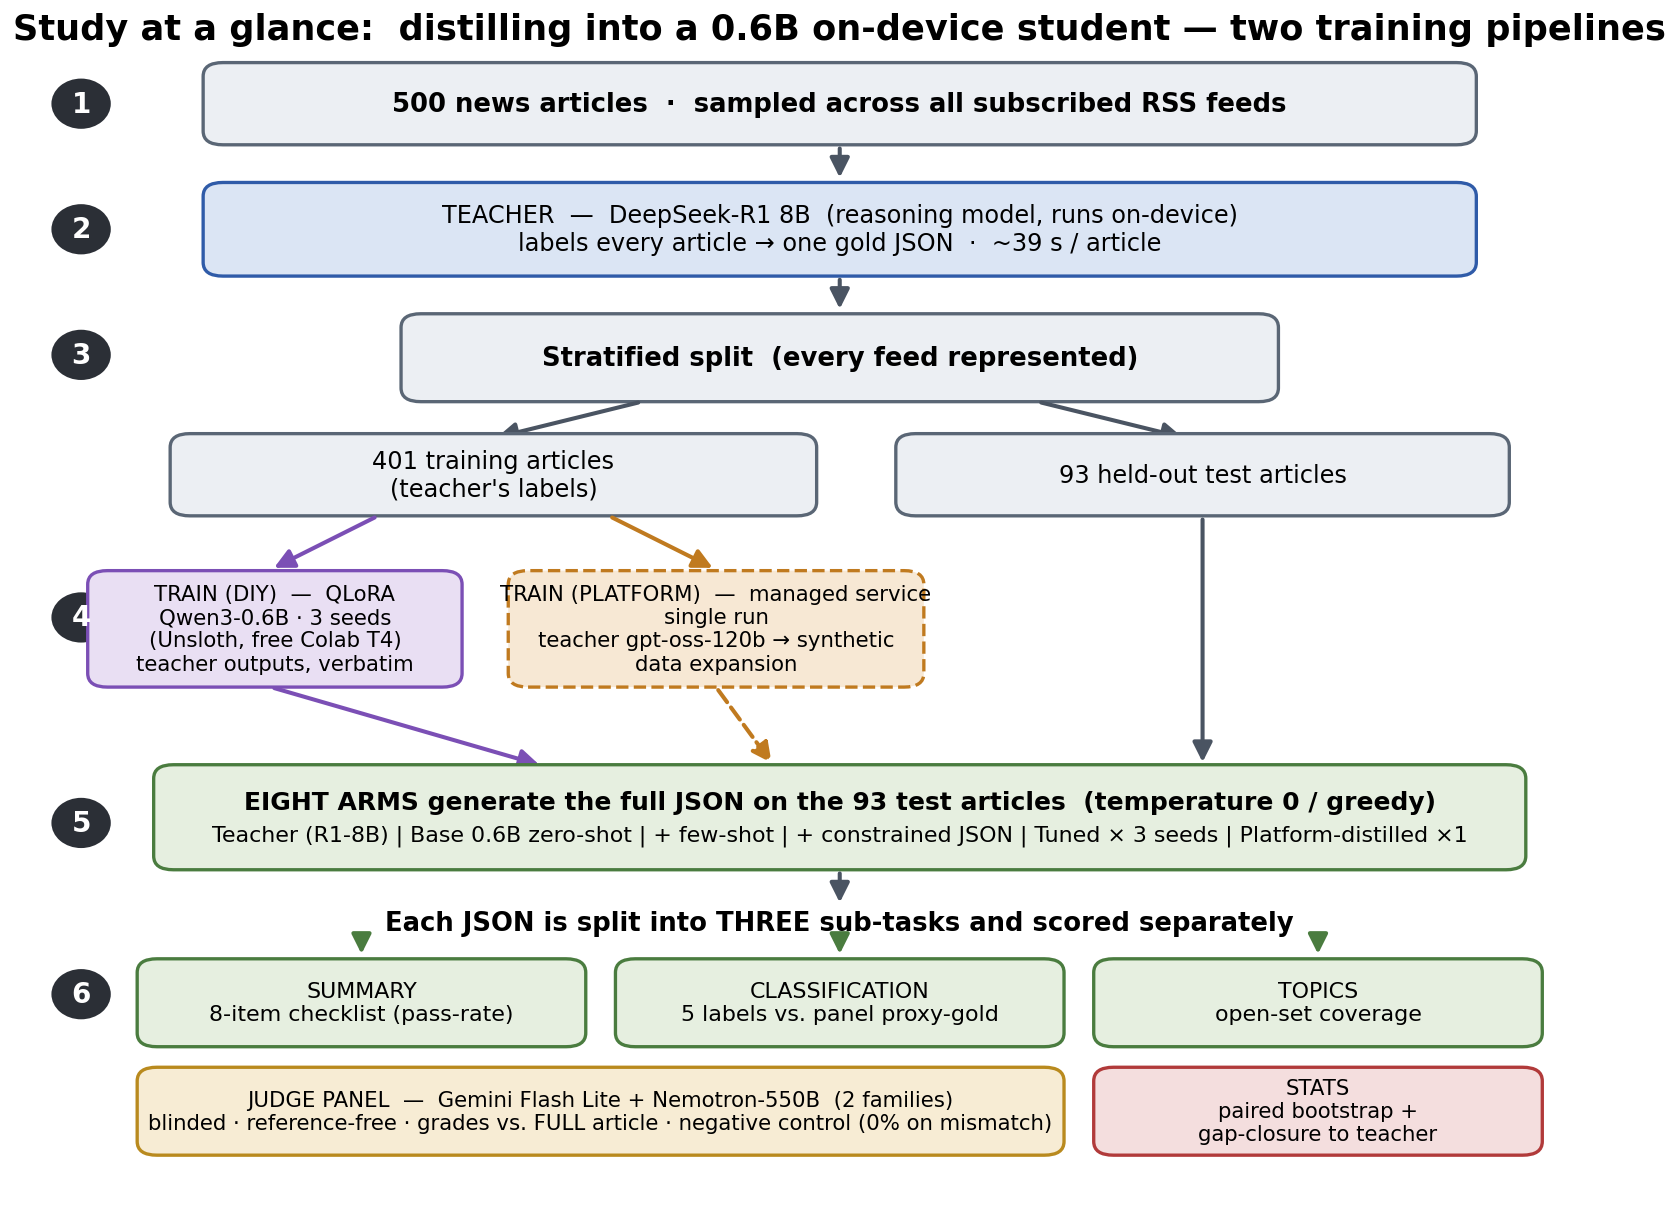
\includegraphics[width=0.92\textwidth]{fig_study_at_a_glance.png}
\caption{The experimental pipeline. 500 articles are labeled by the teacher and split 401/93; the training labels feed two pipelines---the do-it-yourself QLoRA fine-tune (three seeds) and a managed-platform distillation (its own teacher and synthetic-data expansion)---and eight arms generate outputs on the held-out test set; each output is scored on three sub-tasks by a two-judge panel; results are reported as gap-closure toward the teacher.}
\label{fig:glance}
\end{figure*}

\emph{Models.} The teacher is DeepSeek-R1 8B (\texttt{deepseek-r1:8b}); the student is Qwen3-0.6B. Both are served on-device at Q4\_K\_M quantization. A {\raise.17ex\hbox{$\scriptstyle\sim$}}13$\times$ parameter gap and a difference in kind: DeepSeek-R1 emits chain-of-thought before answering, whereas the student is trained on the teacher's final outputs only, compiling task knowledge into weights and skipping runtime deliberation. This choice is deployment-realistic, and it is also why this study cannot separate ``reasoning teacher'' from ``capable 8B teacher'' (Section~\ref{sec:limits}).

\emph{Data and split.} 500 articles sampled fairly across all feeds; the teacher generates a gold JSON for each; malformed outputs are dropped. A stratified-random split gives 401 train / 93 test, every feed represented. The test set is new articles from known feeds---matching deployment (the reader follows fixed feeds and sees new items), not generalization to unseen sources, which is out of scope.

\emph{Training.} A QLoRA fine-tune of Qwen3-0.6B directly on the 401 teacher outputs (LoRA rank 32, response-only loss masking, thinking disabled), on a free cloud T4 GPU. Three seeds (42/123/7) are trained so that seed variance is characterized rather than assumed away. Models are exported to Q4\_K\_M and served locally.

\emph{Arms.} All arms generate at temperature 0 and see the full article. The eight arms are the teacher; the untuned base Qwen3-0.6B; base + few-shot prompting (2--3 in-context examples, controlling for prompting); base + constrained JSON decoding (controlling for formatting); the tuned student at three seeds; and a managed-platform-distilled arm (Section~\ref{sec:platform}) trained from the same 401-item upload through a commercial pipeline with its own teacher (\texttt{openai.gpt-oss-120b}) and synthetic-data expansion, a single run. Distillation is credited only where it beats \emph{both} controls on something real.

\section{Evaluation Method}\label{sec:eval}
\subsection{Metrics per Sub-Task}
\emph{Structure} is schema validity: parses as JSON with all seven fields, computed deterministically. \emph{Classification} is per-field accuracy plus macro-average against a panel-consensus proxy-gold (Section~\ref{sec:judges}; the majority-class baseline of Section~\ref{sec:classification} is the reference line). \emph{Summarization} is an eight-item binary checklist (pass-rate), the primary metric, chosen because a 0--5 rubric saturates; the checks are \emph{faithful}, \emph{thesis}, \emph{takeaway}, \emph{length}, \emph{opening}, \emph{teacher-lens}, \emph{tech-lens}, and \emph{tone}, with a separately reported \emph{topics\_cover} check (full wording in Appendix~\ref{app:checklist}). \emph{Efficiency} is latency, throughput, and memory, measured per-arm. The summary checklist and primary comparison were fixed after a 12-article pilot and before any scored run, so the rubric could not be tuned to the result; two checks were dropped at the pilot for lack of headroom, dropped rather than reworded to avoid post-hoc bias.

\subsection{Judge Panel and Grading}\label{sec:judges}
Grading is reference-free, against the full article, never against the teacher's answer (which would induce teacher-mimicry bias); blinded, with shuffled anonymous arm labels; and at temperature 0. The panel deliberately excludes the teacher's family and the student's family, since a same-family judge can self-prefer. Results come from a two-judge panel, Gemini Flash Lite and Nemotron-550B (two distinct families, $N=93$). Other hosted judges failed mid-run on the free tier and were excluded. Per-check inter-judge disagreement is 26.8\%, so each judge's \emph{direction} is reported independently (Section~\ref{sec:robust}) rather than hidden inside a majority vote. For the classification proxy-gold, where a single label per field is required, ties on the {\raise.17ex\hbox{$\scriptstyle\sim$}}27\% of items where the judges disagree are broken by a fixed judge-priority order; this is a known limitation, since a two-judge ``consensus'' has no true majority on disagreements, so the accuracy numbers should be read as directional (Section~\ref{sec:limits}). Grading uses the full article throughout: partial-context grading systematically understates faithfulness and manufactures an apparent regression, quantified in Section~\ref{sec:robust}.

\subsection{Grader Validation Without Humans}\label{sec:negcontrol}
At this scale, human adjudication is the bottleneck, so the grader is validated by construction: a negative control grades a sample of summaries against a \emph{mismatched} article. A grader that cannot tell a real summary from a mismatched one is not measuring anything. The result is 0\% faithful on mismatched articles ($n=30$): the grader demonstrably discriminates the gross case. It does \emph{not} confirm detection of subtle, in-domain fabrication---a plausible invented detail inside an otherwise-correct summary---which would require injected-fabrication tests or a human-labeled set (Section~\ref{sec:future}). The faithfulness numbers should be read with that boundary in mind.

\subsection{Statistics}\label{sec:stats}
Metrics are reported as mean with 95\% confidence interval (bootstrap over the 93 test items; headline comparisons use a paired bootstrap over per-article scores, 20\,000 resamples, cancelling per-article difficulty). Tuned metrics are the mean across three seeds. The primary comparison, fixed before scoring, is tuned versus base + constrained on checklist pass-rate. Secondary comparisons (tuned versus base, tuned versus few-shot, and the per-field classification comparisons) are numerous, so individual secondary wins not also confirmed by both judges (Section~\ref{sec:robust}) are treated as suggestive. The per-article bootstrap captures article-level variance around the three-seed mean; it does not fully propagate training-seed variance, which Section~\ref{sec:seeds} shows is first-order on the subjective fields---there, the seed range, not the bootstrap interval, is the representative uncertainty.

\section{Results}\label{sec:results}
\subsection{Gap-Closure Toward the Teacher}\label{sec:gapclosure}
Because the goal was teacher quality at student speed, the natural scale is how far the student traveled from the untuned base (0\%) toward the teacher (100\%) on each axis: $(\text{tuned}-\text{base})/(\text{teacher}-\text{base})$. Fig.~\ref{fig:gap} is the paper in one chart. The headline is not one number; it is the \emph{shape}: distillation recovered most of the teacher's quality on most summary axes, exceeded it on two, and left two small summary regressions---faithfulness and length. On classification the picture is more mixed (Section~\ref{sec:classification}). Gap-closure is a ratio and becomes unstable when teacher and base are close, so absolute deltas are reported alongside every gap-closure figure and axes where teacher $\approx$ base are flagged; because the student can exceed 100\% on some axes, the teacher is a reference point, not a ceiling.

\begin{figure}[t]\centering

\includegraphics[width=\columnwidth]{fig3_gap_closure.png}
\caption{Per-axis gap-closure toward the teacher (0 = untuned base, 100 = teacher). Partial recovery, overshoot, and regression below base are distinguished. Distillation recovers most summary and classification axes, overshoots two, and leaves two small summary regressions. The per-axis pattern, not any single aggregate, is the primary result.}
\label{fig:gap}
\end{figure}

\subsection{Summarization}\label{sec:summ}
Checklist pass-rates (Fig.~\ref{fig:checklist}, Table~\ref{tab:checklist}) show a decisive, significant primary win: tuned versus base + constrained is 72.5 versus 57.0, +15.5 points, paired bootstrap $[11.1, 20.3]$, and it holds for each of the three seeds independently. Distillation also beats the prompting control significantly, 72.5 versus 66.7, +5.9 $[2.5, 9.5]$. The summary gain therefore survives both controls a reviewer would demand: it is not reducible to schema formatting or to a few in-context examples. Overall the tuned student closes 59\% of the base-to-teacher summary gap.

\begin{figure}[t]\centering

\includegraphics[width=\columnwidth]{fig4_checklist.png}
\caption{Summary checklist pass-rate by arm, full-text grading, mean with bootstrap 95\% interval ($N=93$). The tuned student significantly beats both non-distillation controls on the paired per-article test. The win rests on the paired comparison, which cancels per-article difficulty, not on marginal-interval separation.}
\label{fig:checklist}
\end{figure}

\begin{table}[t]
\centering
\caption{Summary Checklist Pass-Rate by Arm (Full-Text Grading, $N=93$)}
\label{tab:checklist}
\small
\begin{tabular}{@{}lcc@{}}
\toprule
Arm & Checklist \% & 95\% CI \\
\midrule
Teacher & 84.8 & [81.0, 88.0] \\
Tuned (distilled) & 72.5 & [68.5, 76.3] \\
Base + few-shot & 66.7 & [62.0, 71.2] \\
Base + constrained & 57.0 & [51.9, 61.8] \\
Base zero-shot & 55.0 & [49.5, 60.6] \\
\bottomrule
\end{tabular}
\end{table}

The per-check breakdown (Table~\ref{tab:percheck}) separates the product-critical faithfulness axis from the stylistic ones. Gains are broad---specificity (\emph{takeaway} 44 to 74), the persona lenses, tone, and opening style recover most of the way, and two axes overshoot the teacher. The two soft spots are faithfulness ($-4$) and length ($-2$); the length miss is over-compression, the same style-transfer overshoot that makes the tuned arm fastest (Section~\ref{sec:efficiency}). Because failure costs are asymmetric (Section~\ref{sec:task}), faithfulness is not folded into a single ``the student is better'' headline: the aggregate checklist win is driven by style and specificity while the one product-critical property regressed slightly. That tension is the central result of this section.

\begin{table}[t]
\centering
\caption{Per-Check Summary Pass-Rates and Absolute Deltas}
\label{tab:percheck}
\small
\begin{tabular}{@{}lccccr@{}}
\toprule
Check & Base & Few-shot & Tuned $\mu$ & Teacher & $\Delta$ vs.\ base \\
\midrule
faithful & 79.6 & 83.9 & 75.6 & 93.5 & $-4.0$ \\
takeaway & 44.1 & 47.3 & 74.2 & 89.2 & $+30.1$ \\
teacher-lens & 22.6 & 41.9 & 62.0 & 87.1 & $+39.4$ \\
tech-lens & 36.6 & 44.1 & 54.5 & 63.4 & $+17.9$ \\
tone & 59.1 & 80.6 & 82.8 & 92.5 & $+23.7$ \\
opening & 51.6 & 79.6 & 77.8 & 73.1 & $+26.2$ \\
thesis & 84.9 & 91.4 & 94.2 & 97.8 & $+9.3$ \\
length & 61.3 & 64.5 & 59.1 & 81.7 & $-2.2$ \\
topics\_cover & 87.1 & 95.7 & 95.7 & 98.9 & $+8.6$ \\
\bottomrule
\end{tabular}
\end{table}

\subsection{The Faithfulness Gap}\label{sec:faithful}
Under full-text grading, faithfulness is base 79.6, tuned 75.6, teacher 93.5---the tuned student sits slightly below the untuned base, a $-4$ point gap. Two things resolve what is real. First, the aggregate deficit is within the instrument's noise: the same tuned-versus-base quantity reads $-4.0$ under the seven-arm grading and $-1.5$ under the eight-arm re-grade (Section~\ref{sec:robust}), and the \emph{faithful} check carries $\pm5$--$7$ points of prompt-composition sensitivity. Because the aggregate gap moves by more than half its size when only the prompt packaging changes, the honest claim is direction-consistent but smaller than the instrument's composition noise. Second, what is robust is localized. Splitting by article length, on long articles ($>1200$ chars, $n=71$) the tuned student is level with base (81.7 versus 80.3); the residual regression concentrates in short articles ($\leq1200$ chars, $n=22$), where tuned drops to 56.0 versus base 77.3 ($-21.3$). The sample size warrants caution: $-21$ points on 22 articles, split three ways by seed, is a real but wide signal, best read as ``concentrated in short sources,'' not ``confined to exactly this.'' The mechanism is consistent across seeds: given little article to work with, the student fills the summary with specific-sounding but unsupported claims (Example B, Section~\ref{sec:examples}); on rich source material it stays grounded. For a reader-facing product that cannot tolerate fabrication, even a localized dip is worth routing around (Section~\ref{sec:assignment}).

\subsection{Classification}\label{sec:classification}
Per-field accuracy against the panel proxy-gold (Table~\ref{tab:classification}) is read against a majority-class baseline, because several vocabularies are imbalanced and accuracy below that line is worse than a constant guess. \emph{Urgency} first looked like the standout---the tuned student hits 78.5\%, above every arm including the teacher---but a per-class confusion analysis demotes it: the proxy-gold is heavily skewed (69/93 evergreen, a 74.2\% majority baseline), and the tuned seeds predict evergreen on 79--86 of 93 items (evergreen recall 96--100\%; \emph{developing} 28--33\%; \emph{breaking} 0\%). The student sits +4.3 points above a constant guess: real but modest signal, not learned mastery. No arm ever detects \emph{breaking} ($n=6$). \emph{Frame} shows a smaller version of the same pattern. \emph{Depth} is a caution: at 48.8 the tuned student scores below the {\raise.17ex\hbox{$\scriptstyle\sim$}}56\% of always guessing ``standard,'' and no small-model arm clears the constant-guess line. \emph{Tone} as a categorical label is nearly untouched by distillation (29 versus base 24) while few-shot reaches 79---a field cued far better in-context than baked into weights. On the macro average, distillation ties few-shot (56.0 versus 57.8): on the aggregate categorical task, prompting is as good as fine-tuning, and the distillation advantage is concentrated in \emph{urgency} and \emph{frame}. This is why the deployment recommendation is per-field (Section~\ref{sec:assignment}).

\begin{table}[t]
\centering
\caption{Per-Field Classification Accuracy vs.\ Panel Proxy-Gold}
\label{tab:classification}
\small
\begin{tabular}{@{}lcccccc@{}}
\toprule
Field & Agr. & Maj. & Base & Few & Tuned $\mu$ & Teach. \\
\midrule
urgency & 0.85 & {\raise.17ex\hbox{$\scriptstyle\sim$}}74 & 62.8 & 56.0 & 78.5 & 57.0 \\
frame & 0.86 & --- & 50.0 & 39.6 & 58.1 & 66.7 \\
sentiment & 0.91 & --- & 43.0 & 63.7 & 66.0 & 80.6 \\
depth & 0.70 & {\raise.17ex\hbox{$\scriptstyle\sim$}}56 & 43.0 & 50.5 & 48.8 & 53.8 \\
tone & 0.78 & --- & 24.4 & 79.1 & 29.0 & 78.5 \\
macro & --- & --- & 44.7 & 57.8 & 56.0 & 67.3 \\
\bottomrule
\end{tabular}
\end{table}

\subsection{Structure, Topics, and Efficiency}\label{sec:efficiency}
The tuned student produces valid seven-field JSON reliably, but constrained decoding reaches the same validity with zero training, so structure is a decoding flag, not a reason to distill. Topic coverage is tuned 95.7\% versus base 87.1\% versus teacher 98.9\%, a solid low-stakes gain level with few-shot. On efficiency (Table~\ref{tab:efficiency}, Fig.~\ref{fig:efficiency}), every 0.6B arm runs at {\raise.17ex\hbox{$\scriptstyle\sim$}}0.8 s/article; the tuned model is fastest by wall-clock, not because throughput is higher but because distillation taught it to write shorter outputs. The 5.4 h to {\raise.17ex\hbox{$\scriptstyle\sim$}}7 min batch collapse is real and slightly better for the distilled model than for any other student arm.

\begin{table}[t]
\centering
\caption{Per-Arm Latency and Throughput}
\label{tab:efficiency}
\small
\begin{tabular}{@{}lccc@{}}
\toprule
Arm & p50 (ms) & p95 (ms) & Throughput (tok/s) \\
\midrule
Teacher (R1-8B) & {\raise.17ex\hbox{$\scriptstyle\sim$}}39\,200 & --- & {\raise.17ex\hbox{$\scriptstyle\sim$}}40 \\
Base & 845 & 1434 & 172 \\
Base + few-shot & 856 & 1367 & 154 \\
Base + constrained & 824 & 1422 & 173 \\
Tuned (distilled) & 774 & 1341 & 165 \\
\bottomrule
\end{tabular}
\end{table}

\begin{figure}[t]\centering

\includegraphics[width=\columnwidth]{fig5_efficiency.png}
\caption{Left: batch wall-clock versus volume---the 5.4 h to {\raise.17ex\hbox{$\scriptstyle\sim$}}7 min collapse at 500 articles that motivated the work. Right: the quality-cost plane---every 0.6B arm sits at {\raise.17ex\hbox{$\scriptstyle\sim$}}0.8 s (the horizontal move is free with size); the vertical axis is where distillation, prompting, and the teacher differ.}
\label{fig:efficiency}
\end{figure}

\subsection{Seed Variance}\label{sec:seeds}
The three seeds diverge sharply on the hardest axis: \emph{tone}-label accuracy ranged 8.6\% to 46.2\% across seeds, and classification macro ranged 50.3 to 66.5. A single-seed study could have reported any point in that range as ``the'' result; at 0.6B, seed choice is first-order on the subjective fields, not a rounding error, which is why tuned values are reported as three-seed means. Seed disagreement is also a free confidence signal (Table~\ref{tab:seeds}): where the three seeds agree unanimously, accuracy is 18--43 points higher than where they split, and \emph{tone}, the field distillation fails, is precisely where the seeds almost never agree. Since the three seeds together still run in {\raise.17ex\hbox{$\scriptstyle\sim$}}2.4 s/article, seed-ensemble agreement is a zero-training-cost per-item confidence flag: trust unanimous labels, route split items to a fallback engine (Section~\ref{sec:assignment}).

\begin{table}[t]
\centering
\caption{Seed Unanimity Predicts Label Correctness}
\label{tab:seeds}
\small
\begin{tabular}{@{}lcccc@{}}
\toprule
Field & Unanimous (3/3) & Acc. & Split & Acc. \\
\midrule
urgency & 83 & 83.1 & 10 & 40.0 \\
sentiment & 67 & 73.1 & 26 & 47.4 \\
frame & 57 & 64.9 & 36 & 47.2 \\
depth & 36 & 61.1 & 57 & 40.9 \\
tone & 12 & 50.0 & 81 & 25.9 \\
\bottomrule
\end{tabular}
\end{table}

\subsection{A Managed-Platform Distillation Arm}\label{sec:platform}
A managed-platform pipeline provides a system-versus-system comparison: the same 401 training articles are processed by a commercial service whose pipeline runs its own teacher (\texttt{openai.gpt-oss-120b}), expands the data synthetically, and fine-tunes the same Qwen3-0.6B base in a single hands-off run. Teacher, data recipe, and seed count all differ at once, by design. Adding an arm changes every batched judge prompt, so all arms were re-graded together; the aggregates for the original arms reproduce within 1.6 points (Section~\ref{sec:robust}). The pre-committed primary comparison (Fig.~\ref{fig:platform}, Table~\ref{tab:platform}) is a statistical tie with a do-it-yourself-leaning point estimate: platform versus the tuned mean on the checklist is $\Delta-3.6$, paired bootstrap $[-8.5, +1.1]$. A managed pipeline with a 120B teacher and synthetic-data expansion did not beat a free-tier QLoRA on the teacher's raw outputs on summary quality.

\begin{figure}[t]\centering

\includegraphics[width=\columnwidth]{fig6_platform_checklist.png}
\caption{Summary checklist pass-rate under the eight-arm grading (mean with bootstrap 95\% interval; tuned shown as three-seed mean with seed range). The primary comparison, platform-distilled versus tuned mean, is a statistical tie.}
\label{fig:platform}
\end{figure}

\begin{table}[t]
\centering
\caption{Eight-Arm Grading: The Two Recipes Transfer Different Capabilities}
\label{tab:platform}
\small
\begin{tabular}{@{}lccccc@{}}
\toprule
Arm & Chk. & Faith. & Faith. short & Macro & p50 (ms) \\
\midrule
Teacher & 84.0 & 93.5 & 81.8 & 67.3 & {\raise.17ex\hbox{$\scriptstyle\sim$}}39\,200 \\
Tuned (3-seed) & 71.6 & 72.7 & 53.0 & 56.0 & 774 \\
Platform & 68.0 & 64.5 & 36.4 & 64.3 & 929 \\
Few-shot & 66.8 & 83.9 & 68.2 & 57.8 & 856 \\
Base & 55.1 & 74.2 & 72.7 & 44.7 & 845 \\
\bottomrule
\end{tabular}
\end{table}

The texture is the finding. Direct distillation transferred the teacher's writing: the do-it-yourself arms hold the best small-model summaries (71.6) and the majority-collapsed labels of Section~\ref{sec:classification}. Synthetic expansion transferred label diversity: the platform arm posts the best small-model classification macro (64.3) with genuinely balanced per-class behavior---its \emph{developing} recall is 78\% versus the tuned arms' 28\%, and its \emph{depth} accuracy (62.0) is the first of any arm, including the teacher, to clear the majority-class line. The cost is grounding: the platform arm's faithfulness (64.5 overall) is the lowest measured, and on short articles collapses to 36.4\%, the worst thin-source fabrication in the study, so the synthetic-expansion pipeline appears to amplify exactly the failure mode of Section~\ref{sec:faithful}. The lesson mirrors the paper's thesis one level up: training pipelines, like engines, should be chosen per field.

\subsection{Qualitative Examples}\label{sec:examples}
\emph{Example A, a clean win.} The base model's characteristic failure is to dump the categorical field values into the summary prose (``\ldots The sentiment is positive, with urgency as developing, frame as human\_interest\ldots'') instead of writing a summary. The tuned student instead writes a faithful, correctly structured summary that captures the article's thesis and independently corrects the \emph{urgency} label the base got wrong.

\emph{Example B, the faithfulness cost.} On a short article, the tuned student invents a framing---a subject's presidency described as an ``Obama-style conflict''---that appears nowhere in the source, whereas the teacher stays grounded. This is the residual faithfulness gap of Section~\ref{sec:faithful} in a single instance: a genuine fabrication, the thin-source failure mode isolated statistically, and the reason the routing table (Section~\ref{sec:assignment}) falls back to a more careful engine for faithfulness-critical prose.

\section{Robustness Across Judges}\label{sec:robust}
Inter-judge disagreement is 26.8\% per check, so magnitudes are judge-dependent. But every directional finding in Section~\ref{sec:results} holds under each judge independently: both judges rank tuned above constrained and above few-shot on the checklist, both put \emph{urgency}-tuned above the teacher, and both rank \emph{tone}-label few-shot far above tuned. Only directional claims are therefore made. A third same-family judge was not added because it cannot change a direction the two already agree on; only human gold labels can settle the magnitudes (Section~\ref{sec:limits}).

\emph{Aggregates reproduce; the faithful check shows packaging sensitivity.} Re-grading all arms inside the eight-arm prompts reproduced every checklist aggregate within 1.6 points. The \emph{faithful} check, however, moved $-5.4$ to $-7.5$ points on three arms while remaining unchanged on the others. The cause is not temporal drift: adding a candidate reshuffles the blinded label order in every prompt, so faithful verdicts carry {\raise.17ex\hbox{$\scriptstyle\sim$}}$\pm5$--$7$ points of prompt-composition sensitivity. This is why direction-only claims are made on judge-graded magnitudes.

\emph{Where the disagreement lives.} The \emph{faithful} check has the lowest inter-judge disagreement of all eight (13.7\%) and \emph{thesis} the second lowest (14.4\%): the product-critical checks are the panel's most reliable. Disagreement concentrates in persona and style checks and, strikingly, in two mechanically verifiable checks---\emph{length} (30.6\%) and \emph{opening} (26.3\%). Judges disagree {\raise.17ex\hbox{$\scriptstyle\sim$}}30\% of the time on counting sentences and checking a two-word prefix, a measured noise floor confirming that rule-checkable predicates should be computed by rule. Any verbosity bias runs \emph{against} this study's conclusion, since the winning arm writes the shortest outputs: the tuned student's wins are, if anything, understated.

\emph{Reference-free faithfulness grading must use the full source.} This is the single most transferable methodological result. Grading against only the first 1200 characters produces a $-9$-point faithfulness gap for the tuned student; grading against the full article (the only change) shrinks that to $-4$ and reveals its concentration in short articles (Section~\ref{sec:faithful}). Two checks confirm the artifact: the $+25$--$35$ point full-versus-lead uplift appears for \emph{every} arm (a grading-setup effect, not a model regression), and on long articles the tuned student is level with base. The item-level pattern is stark: moving from lead-only to full-text grading flips 209 faithful verdicts up and only 7 down, every up-flip occurs on articles longer than the truncation point, and short articles---where the two contexts are identical---flip zero verdicts, a built-in negative control. The lesson for reference-free LLM-judge faithfulness evaluation generally: grade against the full source, or a truncation artifact will masquerade as a model regression, here more than twice the size of the real effect.

\section{Per-Field Engine Assignment}\label{sec:assignment}
Judged against the goal of teacher-quality output at student speed: \emph{speed} is fully met ({\raise.17ex\hbox{$\scriptstyle\sim$}}0.8 s/article, 5.4 h to {\raise.17ex\hbox{$\scriptstyle\sim$}}7 min, on-device, at no cost); \emph{summary quality} is substantially met (59\% gap closure, significant wins over both controls), with one localized caveat, faithfulness on short-source articles; \emph{classification quality} is met unevenly (50\% of the gap closed, but the macro only ties few-shot, \emph{tone} barely moves, and \emph{depth} sits below its majority-class baseline). The measured result---and the transferable idea---is therefore not ``use the distilled model'' but a per-field routing map (Table~\ref{tab:assignment}). The map is a measurement deliverable; Section~\ref{sec:design} reduces it to the configuration that should ship.

\begin{table}[t]
\centering
\caption{Per-Field Best On-Device Engine}
\label{tab:assignment}
\small
\begin{tabular}{@{}p{1.9cm}p{2.1cm}p{2.8cm}@{}}
\toprule
Field / output & Best engine & Why \\
\midrule
JSON structure & constrained decoding & free; no training needed \\
urgency, frame & distilled student & best judge agreement; beats both controls \\
sentiment, topics & distilled or few-shot & roughly tied; sub-second \\
depth & platform-distilled & only arm above the majority-class line \\
tone label & few-shot base & prompting far better here \\
summary, long/rich & distilled student & 59\% gap closed; faithful level with base \\
summary, short/thin & teacher (if latency allows) & student fabrication concentrates here (Section~\ref{sec:routing}) \\
\bottomrule
\end{tabular}
\end{table}

The task pattern was chosen because it recurs: the batch collapse is the signature of any high-volume, schema-bound, latency-sensitive enrichment pipeline paying mid- or large-model latency per item---ticket triage (priority + category, the direct analogue of \emph{urgency} + \emph{frame}), log classification, document intake, moderation pre-filters, catalog extraction. For each, the recipe is the same: distill the small model for the structured, high-frequency labels; keep the large model for low-frequency, high-stakes free text; and measure per field rather than assuming the small model wins everything. One task family has been measured; the harness, not this routing table, is the artifact built to transfer.

\subsection{The Routing Table, Scored as a System}\label{sec:routing}
A recommendation assembled from per-field verdicts can and should be scored as a system. Because every arm's output for every test article was individually graded, any deterministic routing rule selects, for each article, an output that already carries grades, so the assembled system's metrics are exact arithmetic over existing per-item scores and the paired-bootstrap machinery applies unchanged. Three summary-routing variants are scored (Table~\ref{tab:routing}; labels always route per-field). The results are: (1) the few-shot fallback for short sources does not work---Router A is indistinguishable from no routing, and its faithfulness moves by less than the instrument's composition noise, so no on-device fallback claims a noise-robust fix; pay the teacher on short sources, or knowingly accept the regression; (2) the teacher-fallback hybrid is a distinct point on the quality-latency frontier---sending only the 22/93 short articles to the teacher buys +5.5 checklist points over all-tuned (paired $[2.7, 8.5]$) and the best faithfulness of any on-device-dominant configuration, at {\raise.17ex\hbox{$\scriptstyle\sim$}}82 minutes per 500 articles; (3) per-field classification routing reaches teacher-level agreement (macro 70.4 versus the teacher's 70.7) at student latency---the strongest quantitative case for treating the field, not the model, as the unit of deployment. These summary-routing differences ride on the 22-article short subgroup, and the routing rules were fixed after seeing the per-field results, so this is engineering validation, not a confirmatory finding.

\begin{table}[t]
\centering
\caption{Routing Configurations Scored as Assembled Systems}
\label{tab:routing}
\small
\begin{tabular}{@{}lcccc@{}}
\toprule
Configuration & Chk. & vs.\ all-tuned & Faith. & Batch \\
\midrule
All-tuned & 71.6 & --- & 72.7 & {\raise.17ex\hbox{$\scriptstyle\sim$}}7 min \\
A: short$\rightarrow$few-shot & 71.2 & $-0.4$ & 76.4 & {\raise.17ex\hbox{$\scriptstyle\sim$}}7 min \\
C: short$\rightarrow$base & 69.6 & $-2.0$ & 77.4 & {\raise.17ex\hbox{$\scriptstyle\sim$}}7 min \\
B: short$\rightarrow$teacher & 77.2 & $+5.5$ & 79.6 & {\raise.17ex\hbox{$\scriptstyle\sim$}}82 min \\
All-teacher & 84.0 & --- & 93.5 & 5.4 h \\
\bottomrule
\end{tabular}
\end{table}

\subsection{From Measurement to Solution Design}\label{sec:design}
The routing map answers a measurement question: which engine is best on each field, and by how much. A deployment answers a different question: which of those wins are worth operating. Measurement should be exhaustive; design should be ruthless. The design rule is the product of three measured quantities: route a field only where (accuracy gain from routing) $\times$ (cost of that field being wrong) exceeds the standing cost of one more engine to version, monitor, and re-evaluate. Applied here, the shipped configuration is two engines and one rule---the tuned student everywhere, a single few-shot pass for \emph{tone} (a $+50$-point gain at low failure cost), with the teacher fallback for thin-source summaries held as a deliberate, latency-priced option---not the full map. That captures most of the measured routing benefit at a fraction of the operating surface. Two costs this harness does not measure are stated plainly: cross-field coherence (nothing enforces agreement between a routed label and the summary), and maintenance surface (every routed engine is one more artifact to re-evaluate on any change). The distinction generalizes: the scientific value of a per-field evaluation is the complete map; the application value is the smallest routed subset that pays.

\section{Discussion and Methods Contribution}\label{sec:methods}
Beyond the routing table, the study contributes a decomposed, reference-free, fully local evaluation harness for structured-output distillation. Each ingredient is individually established in the judging literature (Section~\ref{sec:related}); the contribution is assembling them into a discipline that catches the ways a less controlled evaluation would overstate the method: a per-sub-task decomposition that localizes what distillation moves; gap-closure-to-teacher as a goal-matched reporting scale; two non-distillation controls; the full-source faithfulness-grading result; and human-free grader validation with direction-only multi-judge reporting. The findings came from a chain of build decisions any team distilling for a production task must cross (Table~\ref{tab:decisions}); recording them is much of the exercise's transferable value.

\begin{table}[t]
\centering
\caption{The Decision Surface, as Practitioner Guidance}
\label{tab:decisions}
\small
\begin{tabular}{@{}p{1.7cm}p{5.4cm}@{}}
\toprule
Decision & What the study taught \\
\midrule
Teacher & Output you would ship is the bar; whether its reasoning nature mattered is unresolved (Section~\ref{sec:limits}) \\
Student size & Viable for style, structure, some labels---but seed variance is first-order; budget $\geq3$ seeds \\
Quantization & Measure at the quantization you will ship \\
Tuning recipe & The cheapest recipe moved summary quality decisively; evaluation rigor, not recipe cost, was the bottleneck \\
Training-set size & Enough for style and structure; class balance, not raw count, bound the subjective labels \\
Task framing & The single most consequential evaluation decision: real findings are invisible in the aggregate \\
Controls & Nearly free, and they changed the conclusion twice \\
Judges & Grade against the full source or a truncation artifact masquerades as a regression \\
Ship decision & The unit of measurement is the field; the unit of deployment is the minimal routing that pays \\
Build vs.\ buy & A statistical tie on summaries; the recipes transfer different capabilities---choose per field \\
\bottomrule
\end{tabular}
\end{table}

\section{Limitations}\label{sec:limits}
The reasoning-teacher question is not answered: training used the teacher's final answers only, with no equal-size non-reasoning teacher, so whether the teacher's reasoning nature contributed anything beyond being a capable 8B model is unknown; the framing is scoped to ``an 8B reasoning teacher,'' not to ``reasoning was necessary.'' Labels are silver, not gold: classification accuracy is against a panel consensus, not human truth, so the numbers are judge priors, not ground truth. The two-judge panel leaves magnitudes uncertain and has no true majority on the {\raise.17ex\hbox{$\scriptstyle\sim$}}27\% of items where judges disagree. Faithfulness is reference-free LLM-judged, not entailment-verified, and the negative control validates only the gross case, not subtle in-domain fabrication. The short-article finding rests on a small subgroup ($n=22$). Seed variance is first-order on subjective fields and is not fully propagated by the per-article bootstrap, and the platform arm is a single run without a seed-variance estimate of its own. The pipeline is third-order distillation, which caps the ceiling. Finally, a single task family and feed set is measured; no generalization to unseen sources is claimed.

\section{Future Work}\label{sec:future}
Ordered by expected value: (1) run the equal-size non-reasoning-teacher arm, the one experiment that would answer whether a reasoning teacher helps for non-reasoning tasks at sub-1B scale; (2) add a human-gold anchor on {\raise.17ex\hbox{$\scriptstyle\sim$}}50 items to convert directional magnitudes into settled numbers and calibrate the judges---the single change that would most raise the evidentiary standing of every quantitative claim here; (3) confirm the residual faithfulness gap with a formal entailment verifier and inject-fabrication tests; (4) turn the truncation observation into a measured curve; (5) fix the short-article fabrication mode via faithfulness-filtered data or a decoding-time guard; (6) recover \emph{tone} labeling with a class-balanced training set; and (7) add a reasoning-trace transfer arm.

\section{Conclusion}\label{sec:conclusion}
A distilled 600M student runs the 500-article enrichment in {\raise.17ex\hbox{$\scriptstyle\sim$}}7 minutes instead of 5.4 hours, recovers most of the teacher's summary quality (59\% of the gap) and half of the classification gap, and beats both non-distillation controls on summary quality. The recovery is uneven in ways that matter: on classification the aggregate only ties few-shot prompting, \emph{depth} is untrustworthy for every small-model arm, and on summaries the student transferred the teacher's style and specificity slightly faster than its faithfulness, leaving a small deficit confined to short-source articles. The verdict is therefore not ``distillation works'' or ``distillation hallucinates'' but a two-layer answer: the measurement layer is a per-field map in which every field has a best engine and the winners differ; the design layer is deliberately smaller---ship the tuned student everywhere, one few-shot pass for \emph{tone}, and hold the teacher fallback for faithfulness-critical thin-source prose as a priced option. Two lessons generalize. Decompose before concluding, and check the instrument: scoring the sub-tasks apart made every real finding visible that an aggregate would hide, and grading against the full source rather than a truncated lead turned a $-9$-point ``regression'' into a $-4$-point short-article effect---in reference-free evaluation the measurement setup can be a larger effect than the model. And separate the lever from the goal: speed came from model size, quality-at-that-size from distillation. One question is left open rather than claimed: a reasoning teacher was distilled, but its reasoning was not shown to be the reason it worked. That is the next experiment.

\appendices
\section{Summary Checklist and Judge Prompts}\label{app:checklist}
The checklist (eight binary checks plus topics), graded by the panel against the full article, was fixed after the pilot and before scoring: \emph{faithful} (every factual claim supported by the article); \emph{thesis} (captures the central thesis); \emph{takeaway} (a concrete, specific takeaway); \emph{length} (3--4 sentences); \emph{opening} (does not begin with ``This/The article''); \emph{teacher-lens} (explains a concept accessibly); \emph{tech-lens} (addresses the technical angle); \emph{tone} (direct, contemplative, not alarmist); and \emph{topics\_cover} (the listed topics capture the main themes), reported separately. The checklist judge receives the full article and all arms' summaries under shuffled anonymous labels and returns strict JSON keyed by label. The classification judge assigns exactly one label per field from the closed vocabularies of Section~\ref{sec:task}; the panel vote is the proxy-gold. The negative control pairs each summary with a mismatched article; \emph{faithful} collapses to 0\% ($n=30$).

\section{Reproducibility}\label{app:repro}
All headline metrics recompute offline from the cached judge log, with no API keys. The judge cache holds both the truncated and the canonical full-text responses, keyed by prompt; an environment variable selects which. Released artifacts include the test set with teacher gold, the 401/93 split, per-arm outputs with measured per-item latency, the canonical full-text scorecard, the analysis and paired-bootstrap scripts, and the judge-panel clients.

\section*{Acknowledgment}
The evaluation-harness code, the figure-generation scripts (which render measured data as plots; no figure content is AI-generated), and portions of the manuscript prose were produced with the assistance of AI coding and writing agents. All experimental design, the analysis plan, and the interpretation of results are the author's.

\begin{thebibliography}{99}
\bibitem{hinton2015} G.~Hinton, O.~Vinyals, and J.~Dean, ``Distilling the knowledge in a neural network,'' arXiv:1503.02531, 2015.
\bibitem{kimrush2016} Y.~Kim and A.~M. Rush, ``Sequence-level knowledge distillation,'' in \emph{Proc. EMNLP}, 2016.
\bibitem{xusurvey2024} X.~Xu \emph{et al.}, ``A survey on knowledge distillation of large language models,'' arXiv:2402.13116, 2024.
\bibitem{zhu2023} X.~Zhu \emph{et al.}, ``A survey on model compression for large language models,'' arXiv:2308.07633, 2023.
\bibitem{hsieh2023} C.-Y. Hsieh \emph{et al.}, ``Distilling step-by-step! Outperforming larger language models with less training data and smaller model sizes,'' in \emph{Findings of ACL}, 2023.
\bibitem{li2023} L.~H. Li \emph{et al.}, ``Symbolic chain-of-thought distillation: Small models can also `think' step-by-step,'' in \emph{Proc. ACL}, 2023.
\bibitem{deepseek2025} DeepSeek-AI, ``DeepSeek-R1: Incentivizing reasoning capability in LLMs via reinforcement learning,'' arXiv:2501.12948, 2025.
\bibitem{zhang2025} C.~Zhang \emph{et al.}, ``100 days after DeepSeek-R1: A survey on replication studies and more directions for reasoning language models,'' arXiv:2505.00551, 2025.
\bibitem{li2025} Y.~Li \emph{et al.}, ``NaturalThoughts: Selecting and distilling reasoning traces for general reasoning tasks,'' arXiv:2507.01921, 2025.
\bibitem{aggarwal2025} P.~Aggarwal \emph{et al.}, ``OptimalThinkingBench: Evaluating over and underthinking in LLMs,'' arXiv:2508.13141, 2025.
\bibitem{yang2025} A.~Yang \emph{et al.}, ``Qwen3 technical report,'' arXiv:2505.09388, 2025.
\bibitem{xuspec2024} W.~Xu \emph{et al.}, ``Speculative knowledge distillation: Bridging the teacher-student gap through interleaved sampling,'' arXiv:2410.11325, 2024.
\bibitem{liu2023} Y.~Liu \emph{et al.}, ``G-Eval: NLG evaluation using GPT-4 with better human alignment,'' arXiv:2303.16634, 2023.
\bibitem{ye2023} S.~Ye \emph{et al.}, ``FLASK: Fine-grained language model evaluation based on alignment skill sets,'' arXiv:2307.10928, 2023.
\bibitem{lee2024} Y.~Lee \emph{et al.}, ``CheckEval: A reliable LLM-as-a-judge framework for evaluating text generation using checklists,'' arXiv:2403.18771, 2024.
\bibitem{kim2024} S.~Kim \emph{et al.}, ``Prometheus 2: An open source language model specialized in evaluating other language models,'' arXiv:2405.01535, 2024.
\bibitem{min2023} S.~Min \emph{et al.}, ``FActScore: Fine-grained atomic evaluation of factual precision in long form text generation,'' arXiv:2305.14251, 2023.
\bibitem{ru2024} D.~Ru \emph{et al.}, ``RAGChecker: A fine-grained framework for diagnosing retrieval-augmented generation,'' arXiv:2408.08067, 2024.
\bibitem{tang2024} L.~Tang, P.~Laban, and G.~Durrett, ``MiniCheck: Efficient fact-checking of LLMs on grounding documents,'' arXiv:2404.10774, 2024.
\bibitem{manakul2023} P.~Manakul, A.~Liusie, and M.~J.~F. Gales, ``SelfCheckGPT: Zero-resource black-box hallucination detection for generative large language models,'' arXiv:2303.08896, 2023.
\end{thebibliography}

\end{document}
